\documentclass{article}

%Aus dem LaTex Template der Universit�t Stuttgart
%------------------------------------------------
\usepackage[utf8]{inputenc}
\usepackage[T1]{fontenc}
\usepackage[sfdefault]{ClearSans} %% option 'sfdefault' activates Clear Sans as the default text font
\usepackage{cmap}
\usepackage[ngerman]{babel}
\usepackage{graphicx}
\usepackage[pdftex,hyperref,dvipsnames]{xcolor}
\usepackage{listings}
\usepackage[a4paper,lmargin={2cm},rmargin={2cm},tmargin={3.5cm},bmargin = {2.5cm},headheight = {4cm}]{geometry}
\usepackage{amsmath,amssymb,amstext,amsthm}
\usepackage[lined,algonl,boxed]{algorithm2e}
\usepackage{tikz}
\usepackage{hyperref}
\usepackage{url}
\usepackage[inline]{enumitem} % Erm�glicht �ndern der enum Item Zahlen
\usepackage[headsepline]{scrpage2} 
\usepackage{algorithmic} % F�r Pseudocode
\usepackage{ marvosym } % f�r Pfeil(e)
\usepackage{booktabs} % F�r die sch�neren Booktabs-Tabellen
\usepackage{tikz}
\usepackage{pdfpages}
\usepackage{blindtext}
\usepackage{scrextend}
\usepackage{pdfpages}
\usepackage{natbib} % Yannis hat das importiert; TODO: nachfragen, zu was das gut ist
\pagestyle{scrheadings} 
\usetikzlibrary{automata,positioning}

\begin{document}
	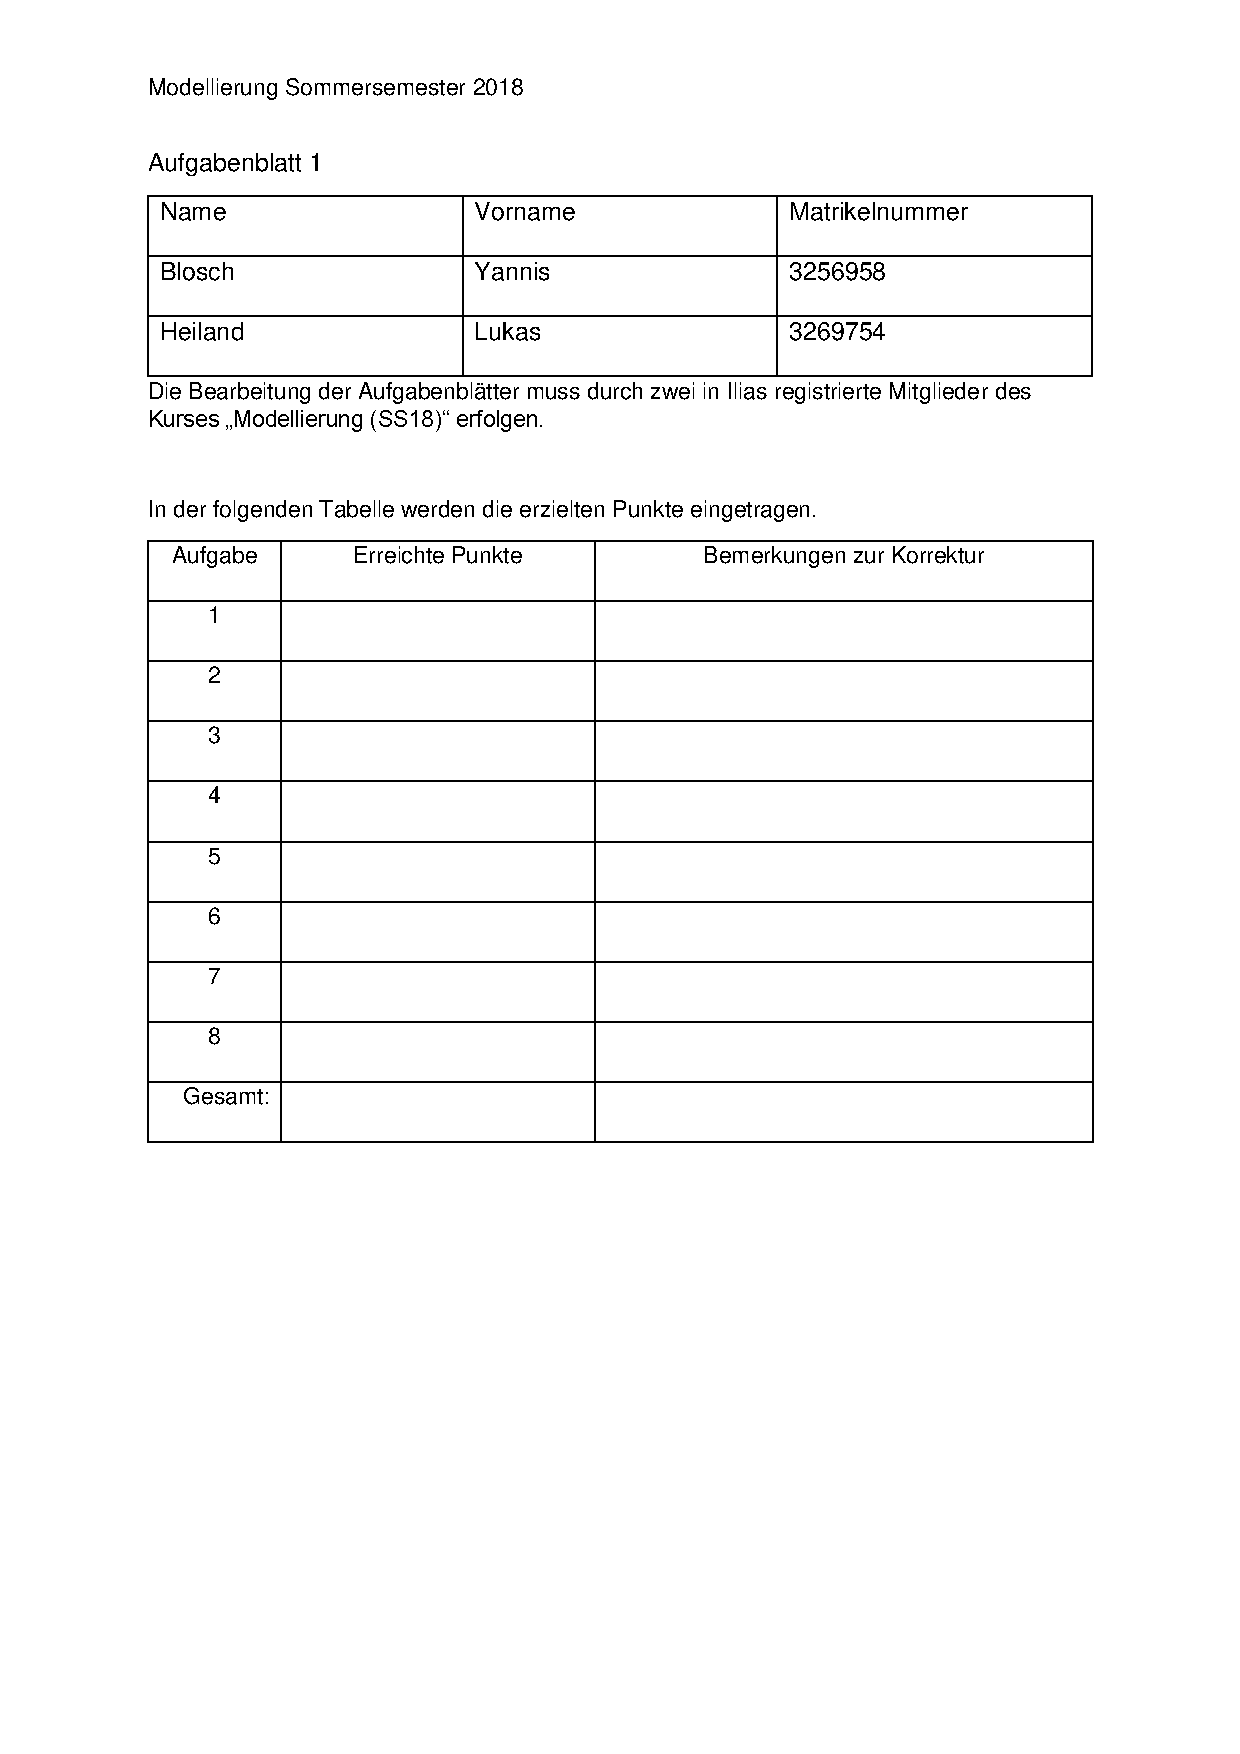
\includepdf[pages=-]{deckblatt.pdf}
	
	% Counter für das Blatt und die Aufgabennummer.
% Ersetze die Nummer des Übungsblattes und die Nummer der Aufgabe
% den Anforderungen entsprechend.
% Beachte:
% \setcounter{countername}{number}: Legt den Wert des Counters fest
% \stepcounter{countername}: Erhöht den Wert des Counters um 1.
\newcounter{sheetnr}
\setcounter{sheetnr}{1} % Nummer des Übungsblattes
\newcounter{exnum}
\setcounter{exnum}{1} % Nummer der Aufgabe

% Befehl für die Aufgabentitel
\newcommand{\exercise}[1]{\section*{Aufgabe \theexnum\stepcounter{exnum} #1}} % Befehl für Aufgabentitel

% Formatierung der Kopfzeile
% \ohead: Setzt rechten Teil der Kopfzeile mit
% Namen und Matrikelnummern aller Bearbeiter
\ohead{Yannis Blosch (3256958)\\
Lukas Heiland (3269754)}
% \chead{} kann mittleren Kopfzeilen Teil sezten
% \ihead: Setzt linken Teil der Kopfzeile mit
% Modulnamen, Semester und Übungsblattnummer
\ihead{Modellierung\\
Sommersemester 2018\\
Blatt \thesheetnr}
	
	\section*{Aufgabe 1.1}
	\paragraph*{a.} Falsch, denn die Kardinalität eines Kapitels ist 1 (eine $1$ auf der Kante zwischen $Buch$ und $enth"alt$) $\Rightarrow$ Ein Kapitel kann nur in einem Buch enthalten sein.
	
	\paragraph*{b.} Richtig. Eine Kardinalität von n bedeutet in Min/Max-Notation nämlich (0,*).
	
	\paragraph*{c.} Falsch, Kapitel können auf derselben Seite beginnen, das Attribut $Startseite$ ist nicht unique.
	
	\paragraph*{d.} Ja, dies ist sinnvoll, denn Kapitel können ohne Buch nicht existieren und lässt sich auch nur mit Hilfe von ihm klar identifizieren.
	
	\paragraph*{e.}Falsch, er kann in (0,*) Fächern Prüfungen abnehmen. Das schließen wir aus dem m.
	
	\paragraph*{f.}Falsch, es wird dafür keine Spezifikation angegeben.
	
	\paragraph*{g.}Richtig, ein Dozent kann einen Studenten mehrfach prüfen, denn die Kardinalität ist m. 
	
	\paragraph*{h.}Falsch, das Attribut $Datum$ ist nicht unique.
	
	\paragraph*{i.}Es sind Kurse mit drei Teilnehmern aber nicht beliebig vielen möglich. Es gilt minimal ein Teilnehmer, maximal 5.
	
	\paragraph*{j.}Falsch, sie können 10 oder mehr Kurse besuchen.
	
	\paragraph*{k.}Falsch, sie müssen mindestens 10 besuchen.
	
	\paragraph*{l.}Falsch, sie muss immer angegeben werden.


	\newpage	
	\section*{Aufgabe 1.2}
	%%% Aufgabenteil a (LHE)
	\subsection*{a.}
	.
	\begin{figure}[h]
		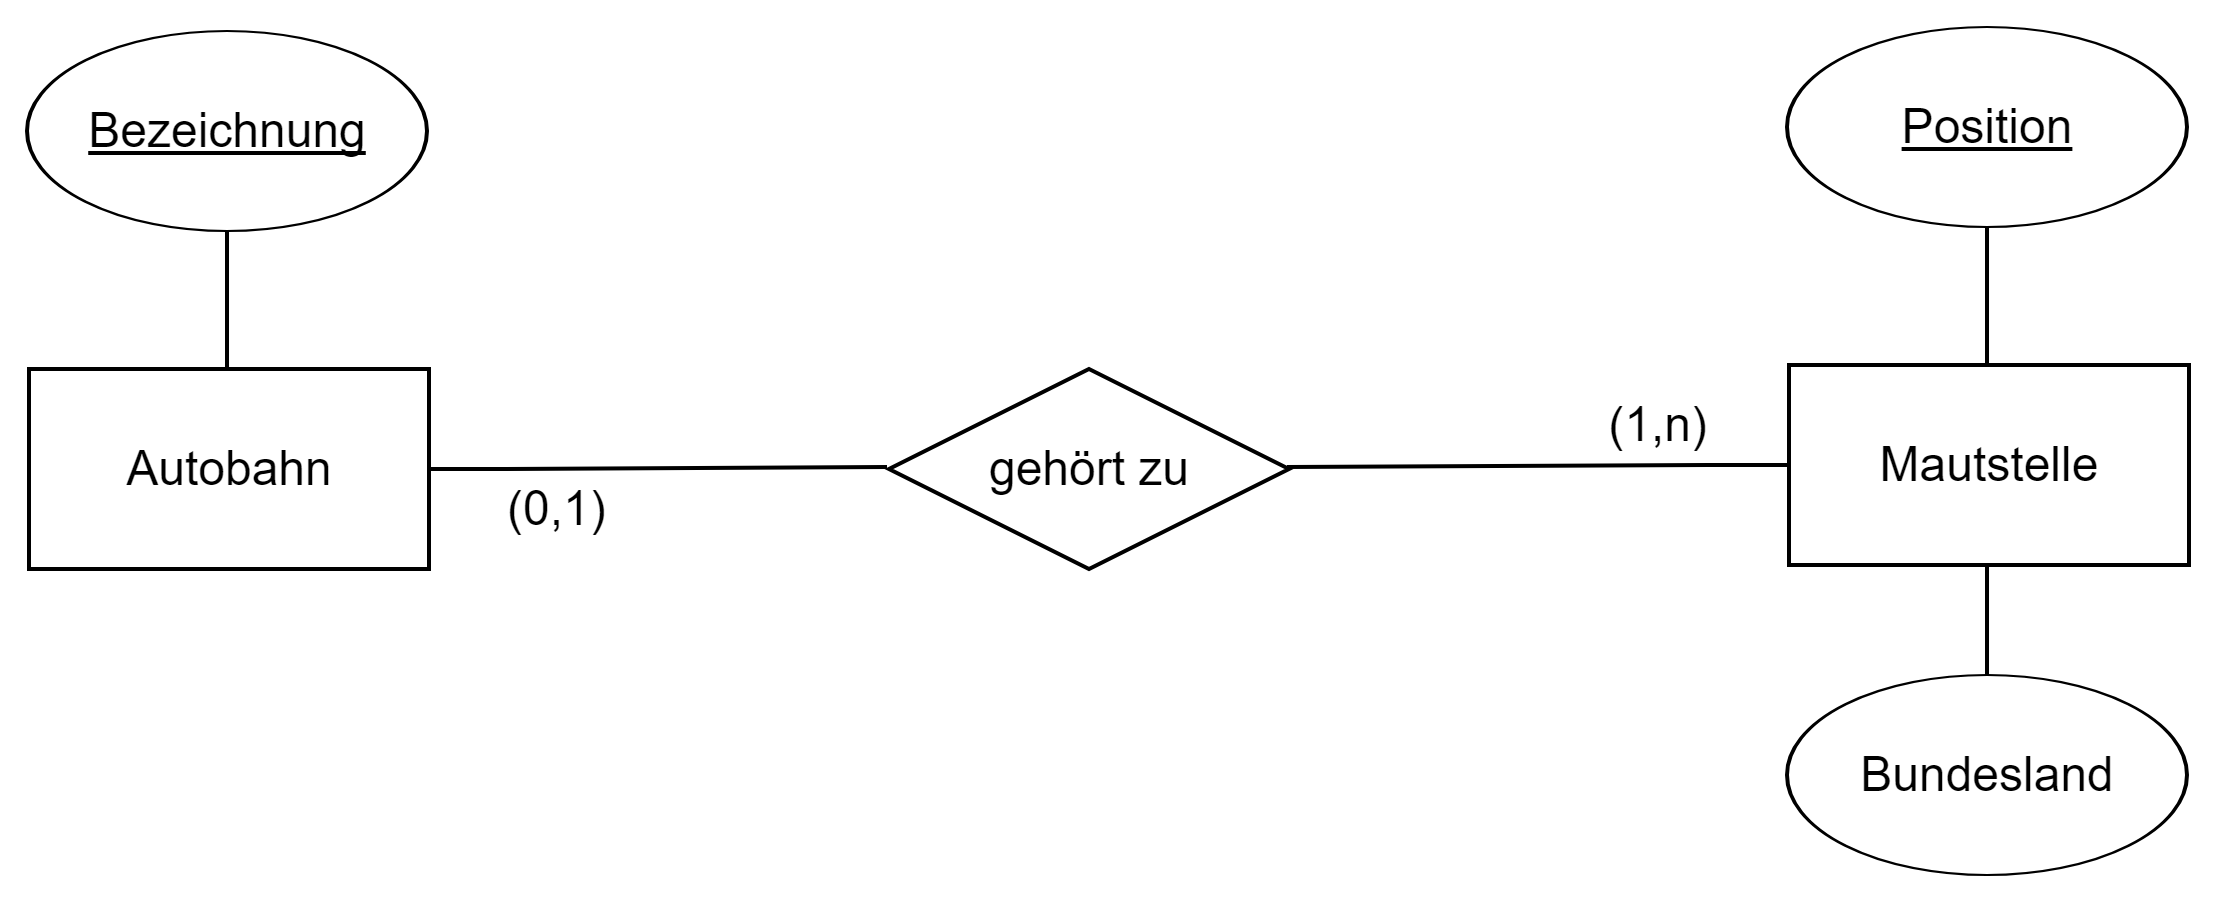
\includegraphics[width=0.7\textwidth]{aufgabe_1_2_a.png}
	\end{figure}
	
	%%% Aufgabenteil b (YBL)
	\subsection*{b.}
	. 
	\begin{figure}[h]
		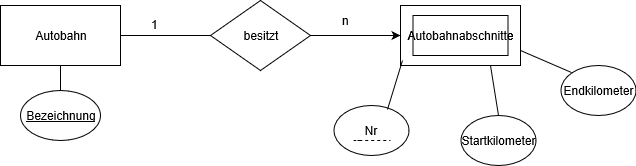
\includegraphics[width=0.7\textwidth]{aufgabe_1_2_b.png}
	\end{figure}
	
	%%% Aufgabenteil c (LHE)
	\subsection*{c.}
	.
	\begin{figure}[h]
		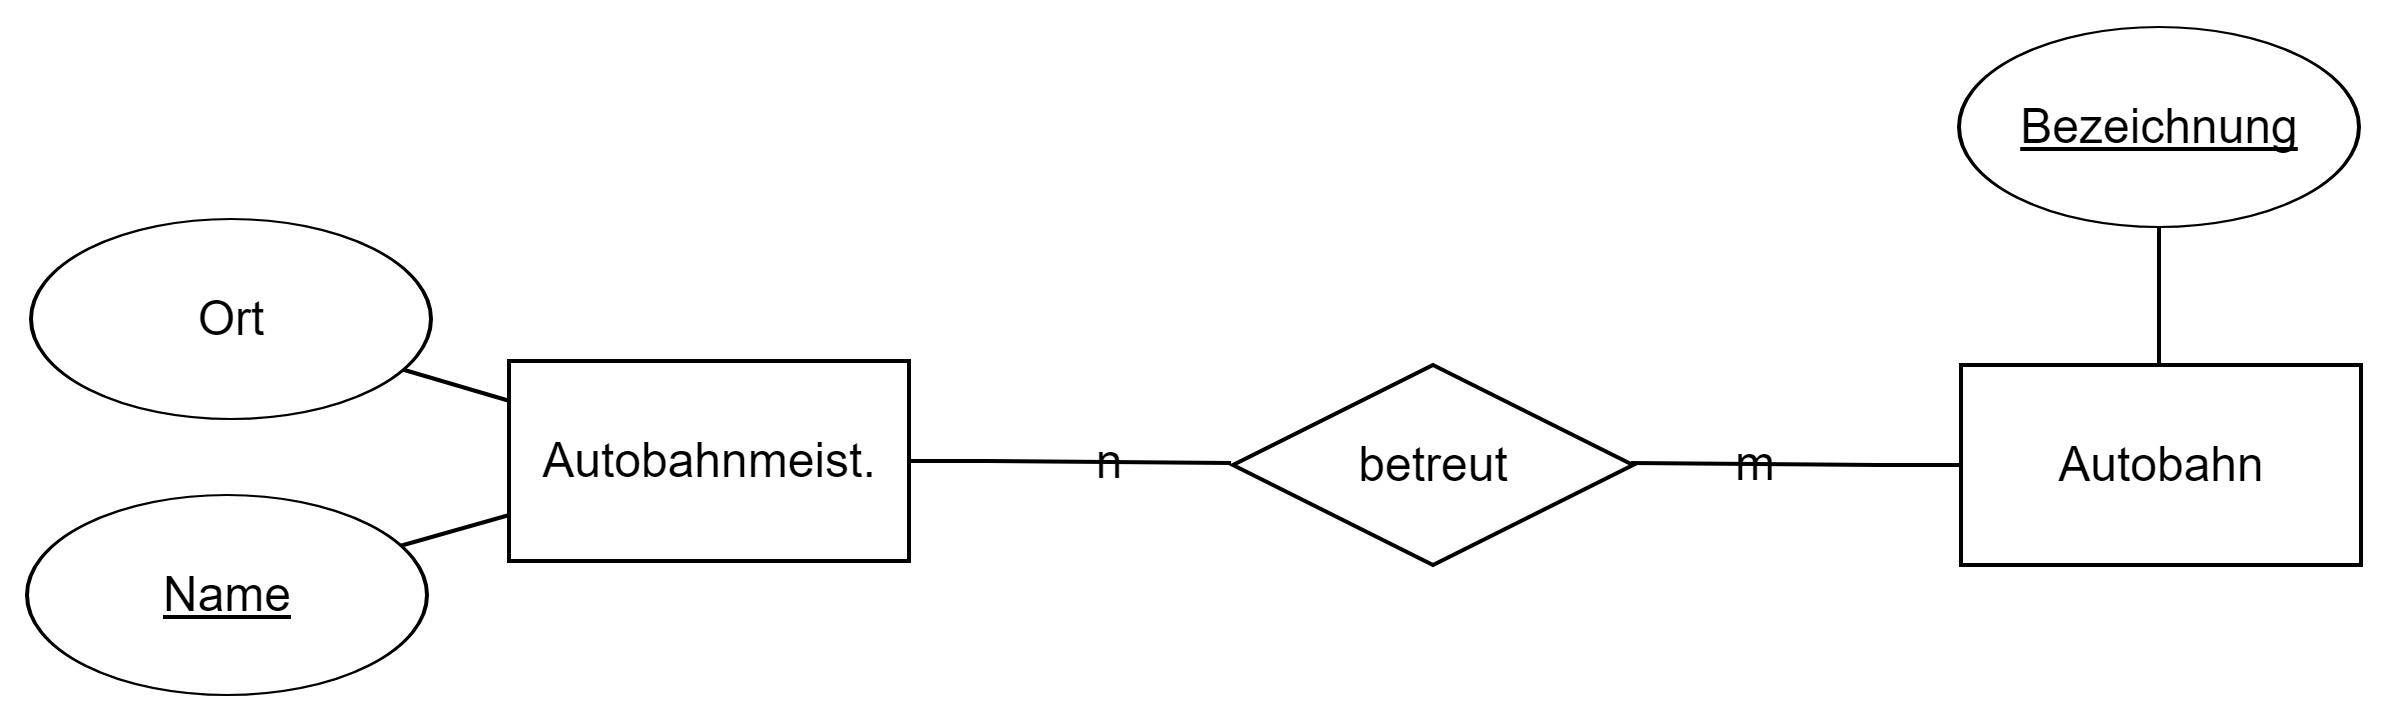
\includegraphics[width=0.7\textwidth]{aufgabe_1_2_c.png}
	\end{figure}
	
	
	\newpage
	%%% Aufgabenteil d (YBL)
	\subsection*{d.}
	.
	\begin{figure}[h]
		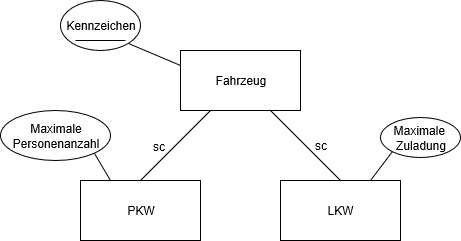
\includegraphics[width=0.7\textwidth]{aufgabe_1_2_d.png}
	\end{figure}
	
	%%% Aufgabenteil e (LHE)
	\subsection*{e.}
	.
	\begin{figure}[h]
		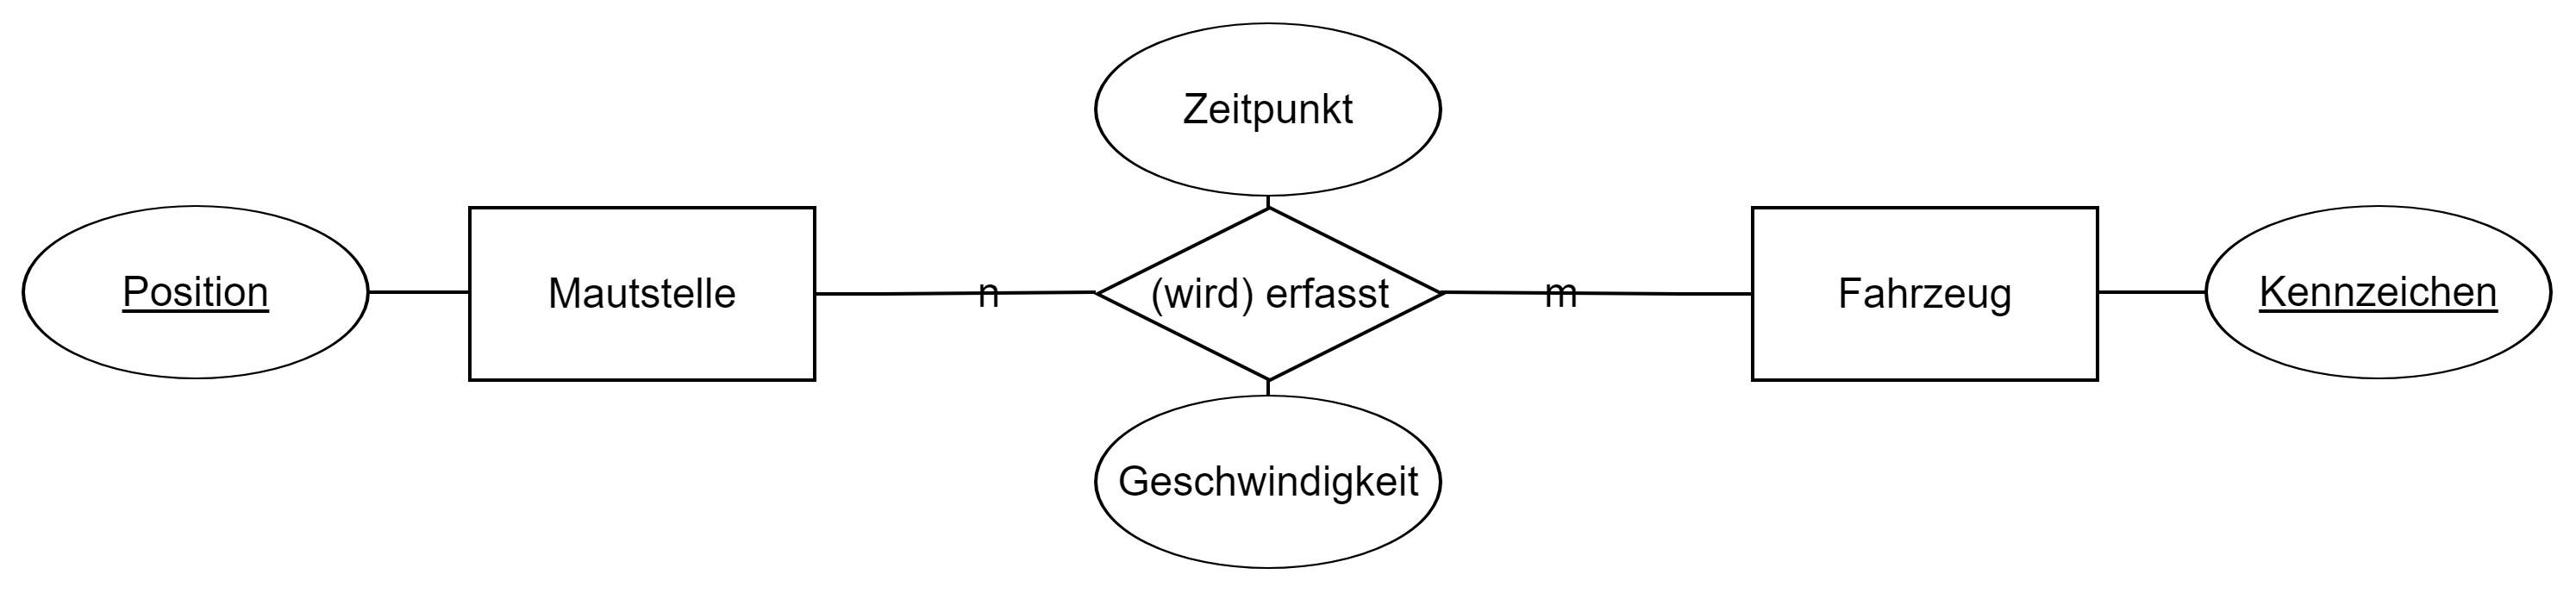
\includegraphics[width=0.7\textwidth]{aufgabe_1_2_e.png}
	\end{figure}
	
	%%% Aufgabenteil f (YBL)
	\subsection*{f.}
	.
	\begin{figure}[h]
		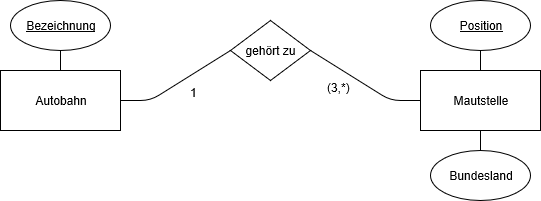
\includegraphics[width=0.7\textwidth]{aufgabe_1_2_f.png}
	\end{figure}
	
	
	%%% layout reasons
	\pagebreak
	
	%%% Aufgabenteil g (LHE)
	\subsection*{g.}
	.
	\begin{figure}[h]
		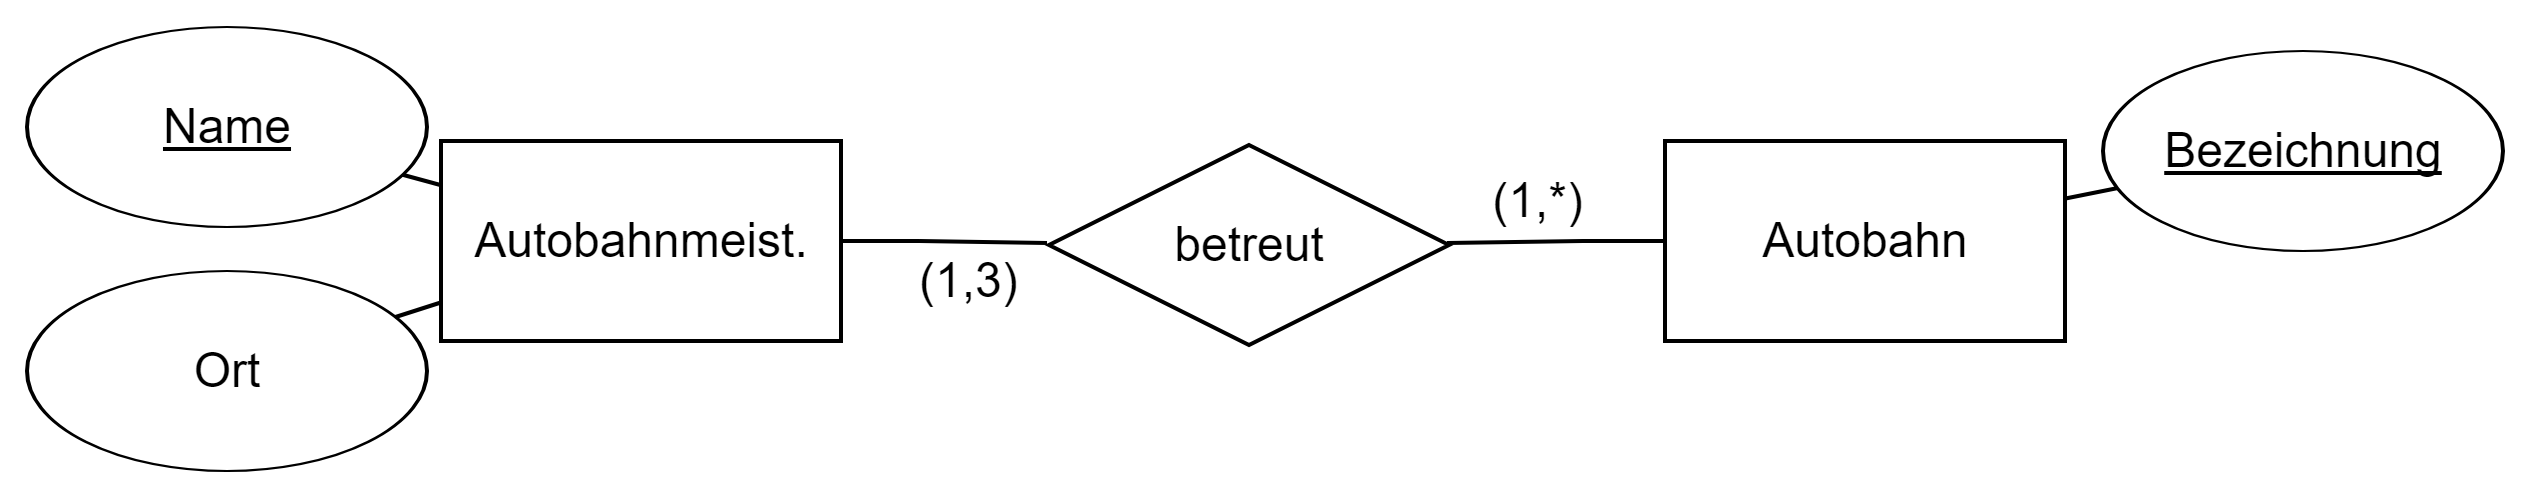
\includegraphics[width=0.7\textwidth]{aufgabe_1_2_g.png}
	\end{figure}
	
	%%% Aufgabenteil h (YBL)
	\subsection*{h.}
	.
	\begin{figure}[h]
		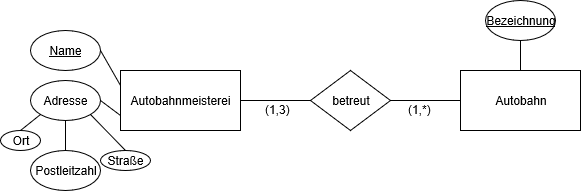
\includegraphics[width=0.7\textwidth]{aufgabe_1_2_h.png}
	\end{figure}
	
\end{document}
